\section{Analysis}
We discuss the benefits of effective localization on issue resolution (\S\ref{sec:downstream_swebench}), the cross-language generalization of \methodname (\S\ref{sec:cross_language}) and evolving tool-use behaviors during RL (\S\ref{sec:tool_use_behaviour}). Appendix \ref{appendix:error_analysis} includes detailed error analysis of \methodname models.



\subsection{Does Effective Code Localization Improve Issue Resolution?}\label{sec:downstream_swebench}
\begin{figure*}[!t]
    \centering
    % Define specific dimensions to ensure uniformity
    \newcommand{\figwidth}{0.49\columnwidth}
    \newcommand{\figheight}{3.3cm} % Adjust this value until the aspect ratio looks natural
        \begin{subfigure}[b]{\figwidth}
        \centering
        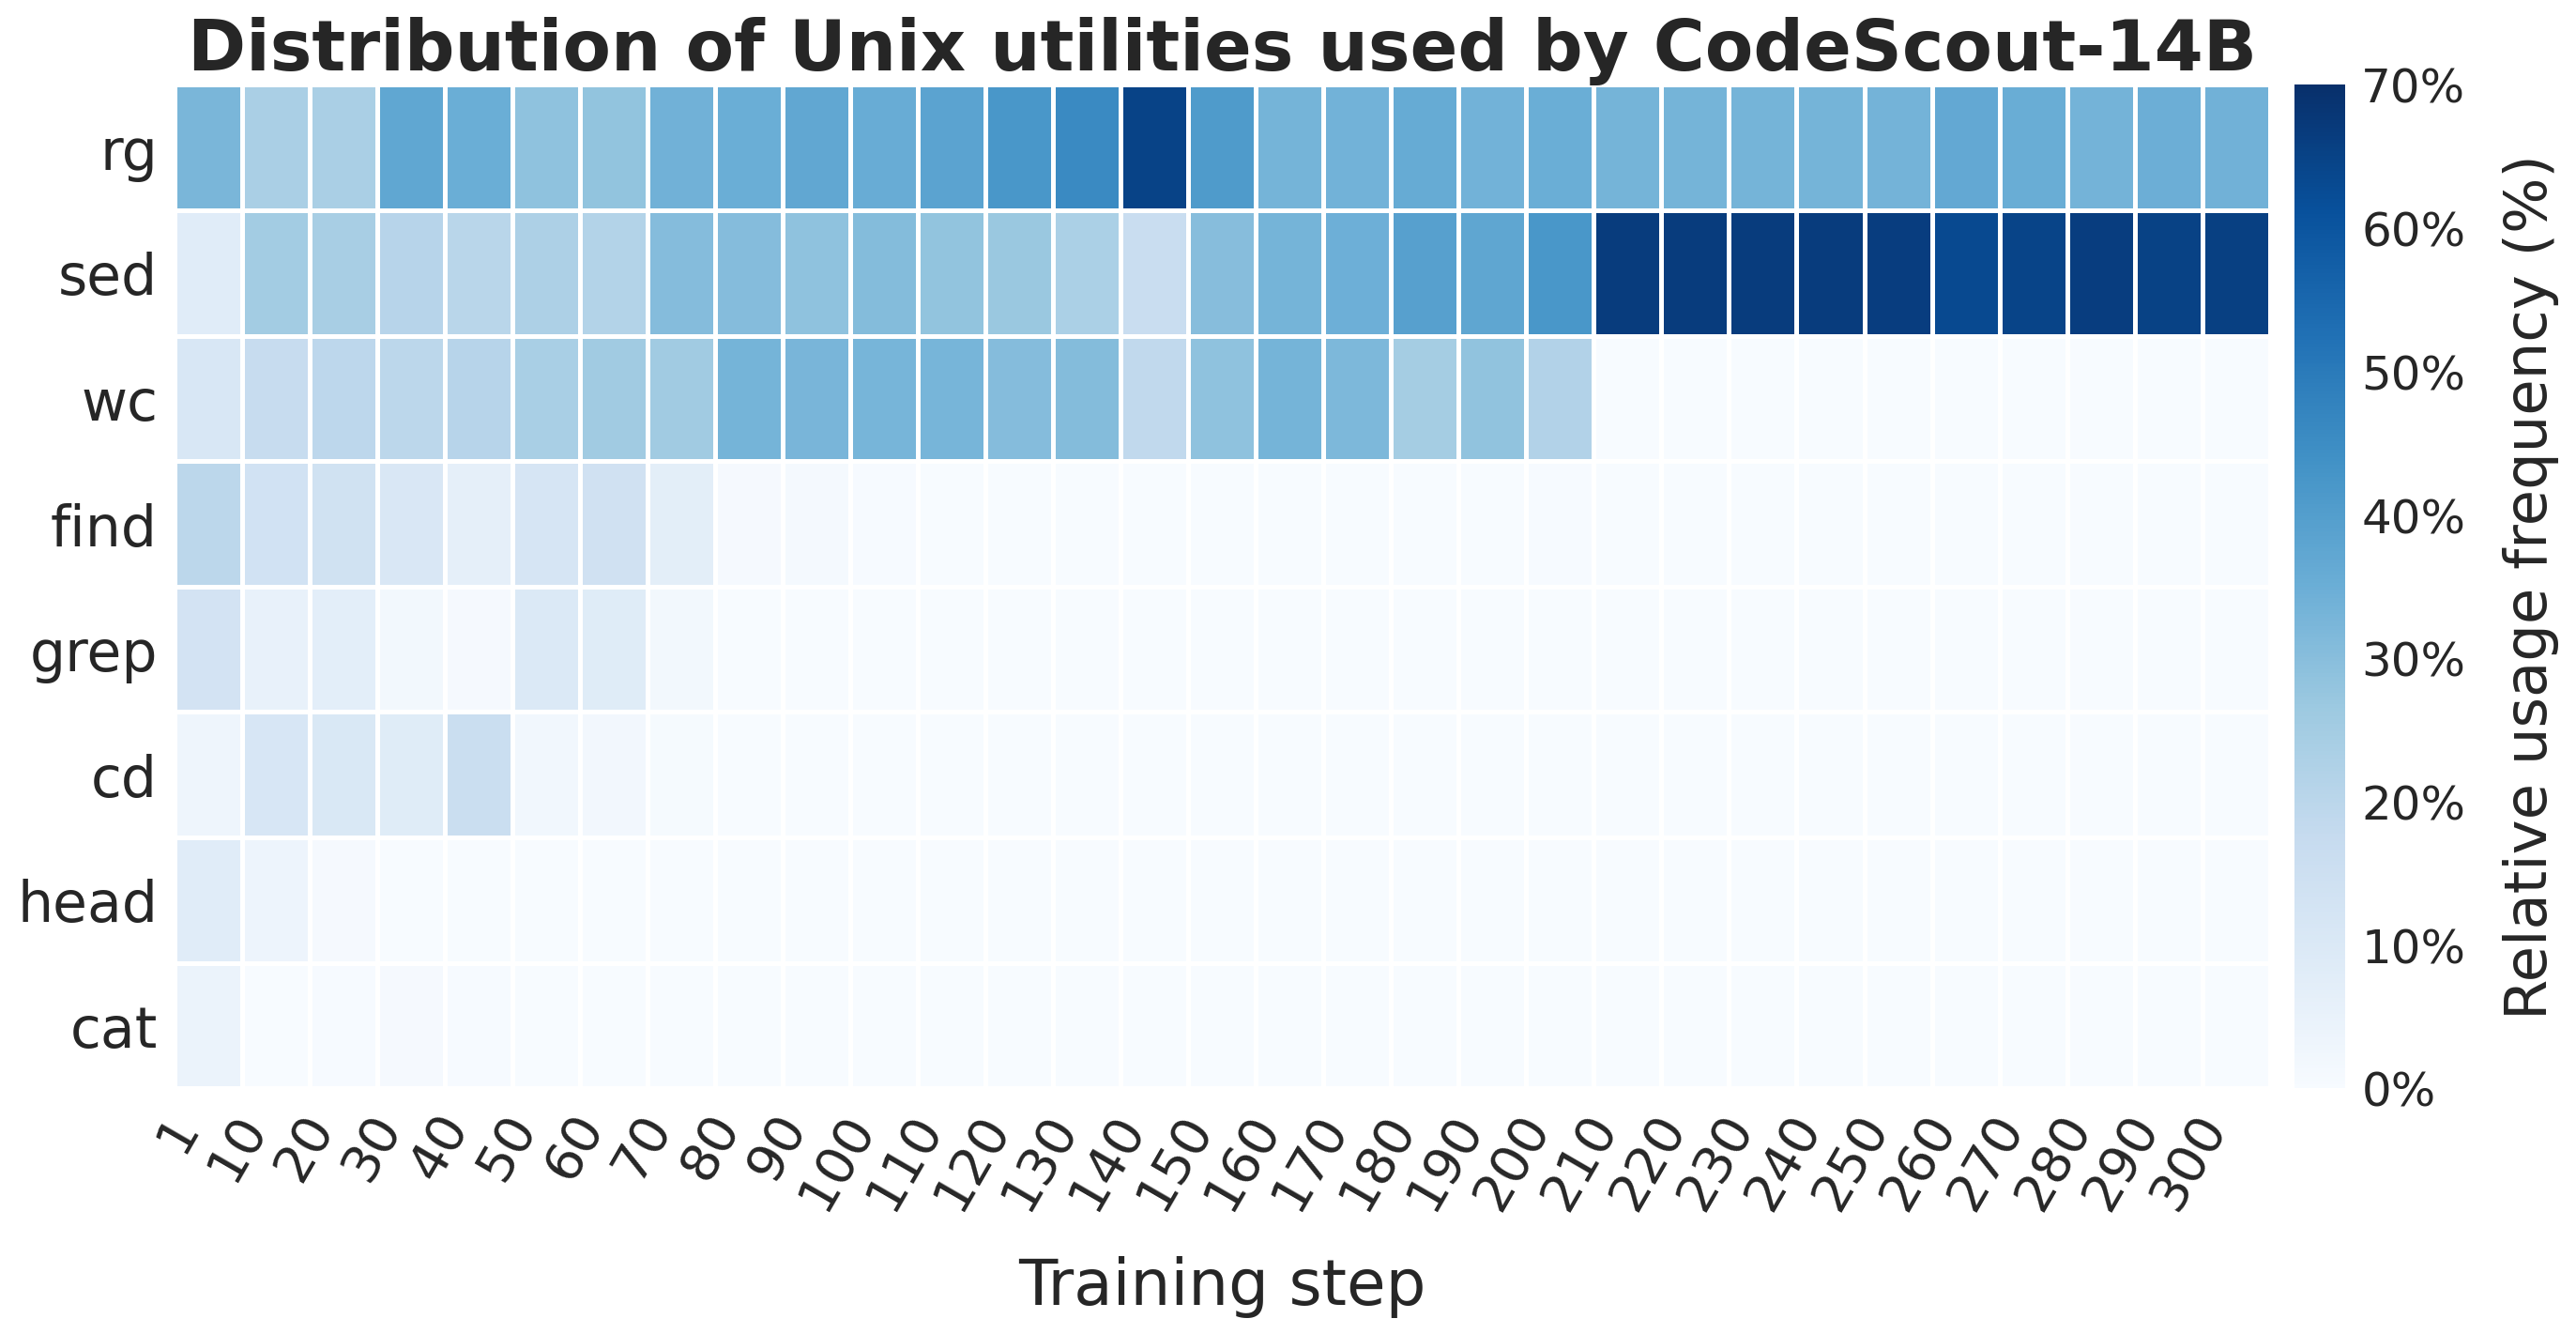
\includegraphics[width=\linewidth, height=\figheight]{Figures/command_relative_freq_14b.png}
        \caption{Tool use for \methodname-14B}
        \label{fig:tool_use_14b_sub}
    \end{subfigure}
    \hfill
    \begin{subfigure}[b]{\figwidth}
        \centering
        % Specifying both height and width forces the images to match exactly
        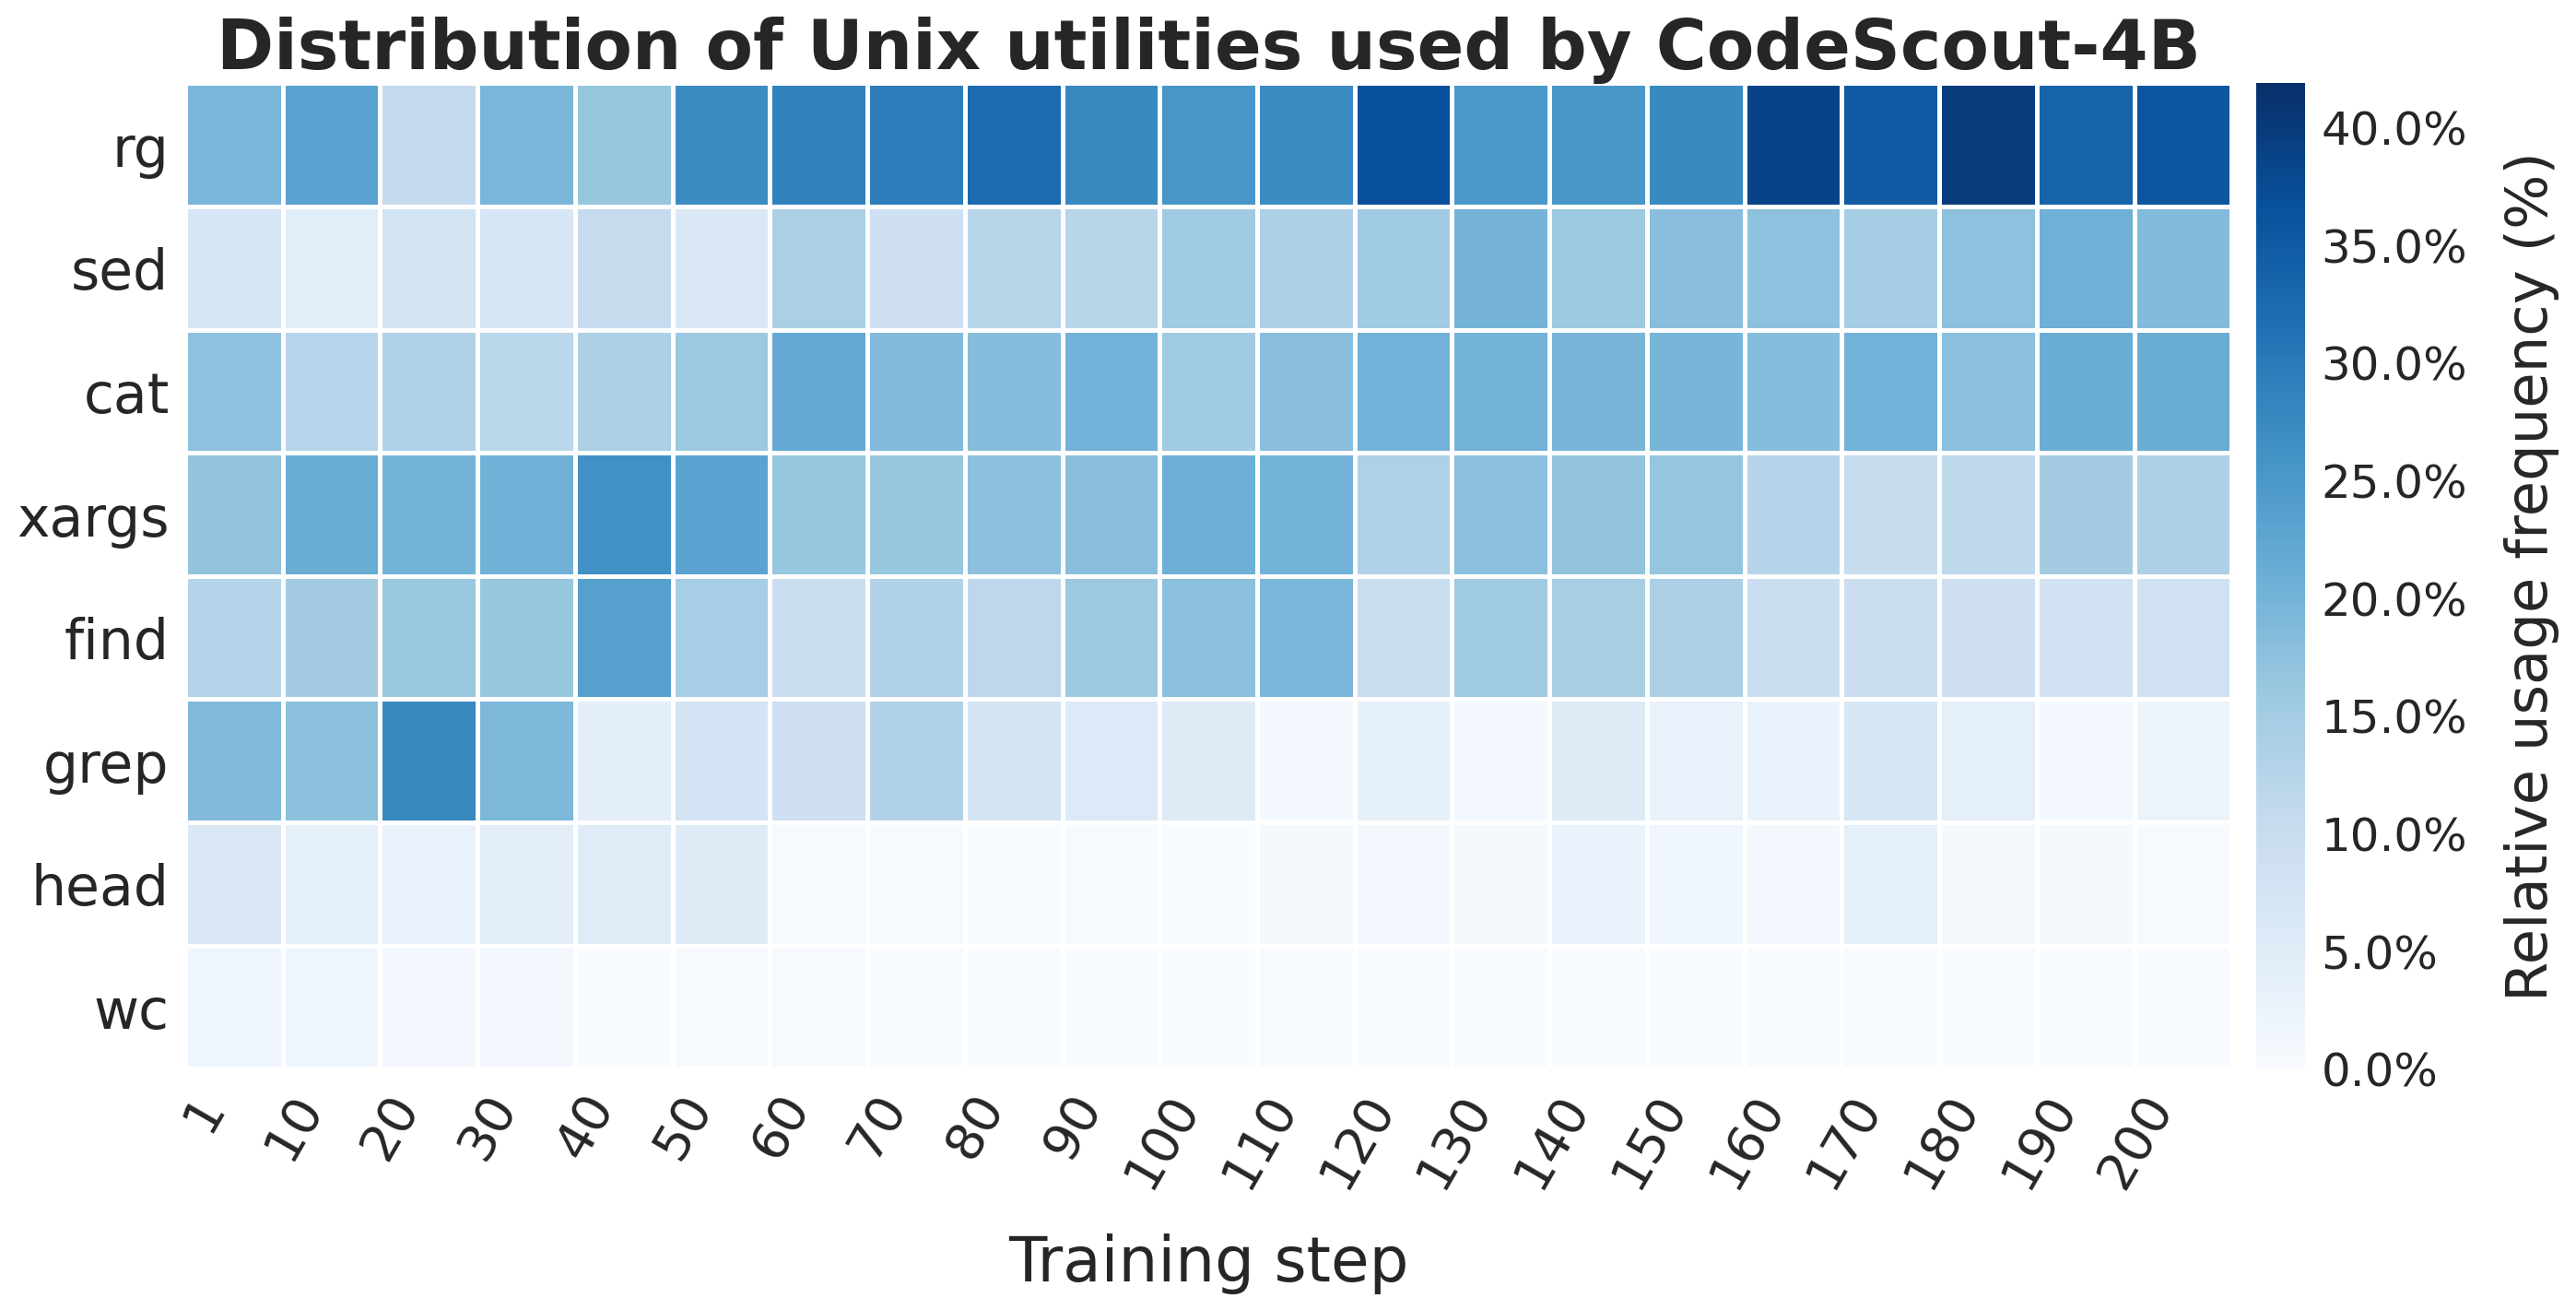
\includegraphics[width=\linewidth, height=\figheight]{Figures/command_relative_freq_4b.png}
        \caption{Tool use for \methodname-4B}
        \label{fig:tool_use_4b_sub}
    \end{subfigure}


    \caption{Distribution of the top-8 most frequent commands used by \methodname. LLMs start with diverse utilities and converge to a small set as training proceeds. \methodname-14B uses only ripgrep (rg) and sed, while \methodname-4B mainly uses rg, cat, sed, and xargs.}
    \label{fig:merged_tool_use}
\end{figure*}
We show that augmenting OpenHands issue resolution agent~\citep{wang2025openhandssoftwareagentsdk} with relevant code retrieved by \methodname improves performance and efficiency on SWE-Bench Verified. We consider three settings: (1) a vanilla baseline without localization, (2) augmenting the agent with locations retrieved by \methodname-14B, and (3) augmenting the agent with oracle locations from the gold patch (\S\ref{sec:data_creation}). 
For (2) and (3), the user prompt is modified to include the locations of relevant files, modules, and functions (Appendix~\ref{appendix:prompts_swe_bench}). We evaluate Qwen3-4B-Instruct-2507 and Qwen3-Coder-30B-A3B-Instruct and report \% of issues resolved, number of steps per trajectory and the total input and output tokens accumulated across all turns in Table~\ref{tab:downstream_swe_bench}.
  
\begin{wraptable}{r}{0.5\columnwidth}
    \centering
    \caption{Issue resolution performance on SWE-Bench Verified: augmenting the agent with relevant locations improves performance and efficiency. Best metric is \textbf{bold-faced} and 2$^{nd}$ best is \underline{underlined}.}
    % \vspace{-15pt} % Adjust vertical alignment as needed
    \resizebox{0.5\columnwidth}{!}{%
        \renewcommand{\arraystretch}{1.1}
        \begin{tabular}{lcccc}
        \toprule
        \makecell[l]{\textbf{Localization }\\\textbf{Approach}} & \makecell{\textbf{Resolution}\\\textbf{Rate $\uparrow$}} & \makecell{\textbf{Avg. \# }\\\textbf{Steps $\downarrow$}} & \makecell{\textbf{Avg. Input}\\\textbf{Tokens $\downarrow$}} & \makecell{\textbf{Avg. Output}\\\textbf{Tokens $\downarrow$}} \\
        \midrule
        \multicolumn{5}{c}{\textbf{Qwen3-4B-Instruct}} \\
        \midrule
        None (Vanilla) & 13.40\% & \underline{16.09} & 344.37K & \underline{2.98K} \\
        \methodname-14B & \underline{17.20\%} & \textbf{13.91} & \textbf{284.26K} & \textbf{2.78K} \\
        Oracle & \textbf{19.60\%} & 16.41 & \underline{327.75K} & 3.17K \\
        \midrule
        \multicolumn{5}{c}{\textbf{Qwen3-Coder-30B-A3B-Instruct}} \\
        \midrule
        None (Vanilla) & 45.20\% & 51.00 & 1596.71K & 13.49K \\
        \methodname-14B & \underline{46.00\%} & \underline{48.11} & \underline{1511.53K} & \underline{13.22K} \\
        Oracle & \textbf{52.00\%} & \textbf{46.74} & \textbf{1358.60K} & \textbf{12.48K} \\
        \bottomrule
        \end{tabular}%
    }
    \label{tab:downstream_swe_bench}
    % \vspace{-15pt}
\end{wraptable}
For Qwen3-4B-Instruct, augmenting the agent with \methodname-14B's outputs improves resolution rate by \textbf{3.8\%}, while reducing trajectory length by \textbf{2.18} steps, and input and output tokens by \textbf{17.46\%} and \textbf{6.71\%} respectively.  Similar efficiency gains are observed for Qwen3-Coder-30B-A3B-Instruct, with \textbf{2.89} fewer steps and \textbf{5.33\%} fewer input tokens and \textbf{2.00\%} fewer output tokens, while achieving comparable performance (+0.80\%). For both LLMs, replacing \methodname predictions with oracle locations yields further performance gains, and the 30B model also benefits with improved efficiency. Thus, continued improvements in localization further improve performance and efficiency of issue resolution agents. Appendix \ref{appendix:localization_quality} shows fine-grained performance breakdown with respect to CodeScout-14B's localization quality.

\subsection{Does \methodname Generalize Across Programming Languages?}\label{sec:cross_language}
We show that the performance improvements of \methodname over their base models generalize to programming languages other than Python, despite our RL post-training using Python-only repositories. We evaluate \methodname-4B and 14B, and their corresponding base models, on the 465 non-Python instances in SWE-Bench Pro, that include Go, JavaScript, and TypeScript,  using our language-agnostic OpenHands-Bash scaffold with a similar evaluation setup from \S\ref{sec:eval_benchmarks}. Since the patch processing scripts from LocAgent \citep{chen-etal-2025-locagent} only support Python, we do not have ground truth functions and modules edited by the patch, and only report file-level localization performance ignoring functions and modules predicted from the model. 

\methodname-4B improves file-level F1 from 17.38 to \textbf{32.56}, while \methodname-14B improves from 19.41 to \textbf{22.99}. These results provide evidence that the learned localization behavior transfers across programming languages, while our Unix-terminal-based scaffold requires no language-specific engineering. All specialized baseline scaffolds from \S\ref{sec:eval_benchmarks} require additional engineering to perform localization on languages other than Python.

\subsection{How does the tool-use behaviour of \methodname evolve during RL?}\label{sec:tool_use_behaviour}
To analyze the evolving tool-use behaviors during RL, we plot the distribution of Unix utilities invoked by the LLM in Figure~\ref{fig:merged_tool_use}. We parse rollouts sampled from model checkpoints at every 10 training steps and aggregate command usage across these checkpoints to identify the top-8 frequently used commands. For each checkpoint, we compute the relative usage frequency of each utility for all rollouts logged in that training step.

We observe convergence in tool usage during RL. While the 14B LLM initially uses various utilities, after 200 training steps it uses \emph{only} two commands: \texttt{ripgrep} (\texttt{rg}) and \texttt{sed}. Similarly, while the 4B LLM initially uses many utilities, it converges to mainly using \texttt{ripgrep}, \texttt{sed}, \texttt{cat}, \texttt{find} and \texttt{xargs}. Thus, we can further simplify the agent to a small subset of Unix utilities without needing access to the entire terminal which is crucial in security-sensitive deployments. Appendix~\ref{appendix:traj_examples} presents example trajectories for 4B and 14B LLMs. 
% We provided analysis of evolving tool-use behaviours of \methodname-4B and \methodname-14B during their respective RL training runs. For all training steps, we parse the Unix utilities from the raw commands issued by the agent when using the \texttt{Terminal} tool across all turns in each sampled rollout. We restrict our analysis to the top-8 Unix utilities based on their total usage frequency across over the entire training run. Finally, we plot the heatmap of the relative usage frequencies of these utilities for every 10 training steps, 

% In Figure \ref{fig:merged_tool_use}, we observe that at the start of training, \methodname tries out multiple different bash commands such as \texttt{cat}, \texttt{grep}, etc. However, as training progresses, the agent quickly converges to using less command variations and after 250 steps only uses \texttt{rg} and \texttt{sed}. This is most likely due to the \texttt{rg} command being comprehensive enough as functionalities from \texttt{cat}, \texttt{find}, and \texttt{grep} can be done with \texttt{rg}. \texttt{cd} also sees dimishing use likely due to the the more effective use of \texttt{rg} that makes changing directory unnecessary.